\documentclass[a4paper,10pt,twocolumn]{article}
\usepackage{amsthm}
\usepackage{listings}
\usepackage{hyperref}
\usepackage{graphicx}
\lstnewenvironment{php}{\lstset{language=php}}{}

\newtheorem*{definition}{Definition}

%opening
\title{Graduate Project Proposal: \\ Dead code elimination in object oriented, dynamic and weakly typed languages}
\author{Hidde Boomsma \\ Faculty EEMCS, Delft University of Technology \\ Delft, The Netherlands}

\begin{document}
\maketitle

\section{Introduction}
At Hostnet PHP\footnote{\url{http://www.php.net}} is used to build complex web applications. Within the company the need rose to delete old program code from the application to make it easier to go forward. Before it is possible to discuss the possible solutions in depth we first have to define what we mean by dead code and see what properties the language and the application at hand possesses.  

\subsection{Dead code}

\subsubsection*{What is dead code?}
The research is about dead code, but the terminology dead code is not very well defined in literature. Sometimes dead code means code that is unnecessarily executed \cite{knoop1994}, in other cases all code that could never be executed because it is never called upon, is called dead\cite{chen1998}. Others call this code unreachable\cite{janota2007} and the former redundant code\cite{biggar2010}.

Because of the ambiguity of the term dead code we define it to mean the following:
\begin{definition}[dead code]
All code that is never executed by a running program but part of the distribution. This includes unreachable code and code for unused features. This does not include redundant code because this code is executed. For a dynamic language this also includes all unused source files.
\end{definition}


This leaves us with two subclasses of dead code unreachable code and unused code. Unreachable co\-de is well defined and in simple terms means:

\begin{definition}[unreachable code]
Code that could never be executed because there is no possible control flow that will lead to the execution for that piece of code.
\end{definition}

As last type we define the unused code:

\begin{definition}[unused code]
Unused code is code that is reachable but is never executed. 
\end{definition}
This type of code could not be found without running the application because it depends on the user if the code will be executed or not.


\subsubsection*{Where does dead code come from?}

Dead code can have thee causes:

\begin{enumerate}
\item Unclear or incomplete specifications
\item Programming mistakes
\item Features that are not used any more
\end{enumerate}

Unclear specifications leads to dead code when pieces of code are only ran when certain conditions are met. If those conditions are never met in practice because such a case will never arise, those pieces of code are written for nothing due to unclear or incomplete specification.

Programming mistakes are always made, also in the initial writing of a program. But most arise when changing the software to add new functionality or repair bugs. Changing a program will often lead to decay of the structure of an application\cite{parnas1994}. Which in turn will lead to more dead code because programmers are always weary about removing code when they do not have a clear view of the whole program.

Dead code because of unused features is a common pattern when software ages. The programmers do not know that certain features are abandoned or simply do not dare remove them\cite{parnas1994}. When it is known that features are not used any more removing them is not a trivial matter because other parts of the application may have common code with the unused feature. A deep knowledge about the application is required to do so.

\subsubsection*{Why is it a problem?}

Dead code is a problem because it will lead to bigger applications. Bigger applications require more memory and take longer to load. But these are not the major problems.

The big problem is that adding features to a big application consumes more precious programmer time than to a little application\cite{godfrey2000}. This is because one needs to understand an application before functionality can be added in the right place. This is also a second problem, how bigger the application the easier code is misplaced or even dead code is resurrected unintended.

In general dead code will make a application harder to maintain. Dividing an application in smaller independent modules with a clear defined makes adding functionality easer\cite{godfrey2000}, but also eases the dead code detection because analysis could be done on the smaller modules.

\section{Dynamic languages}
\label{sec:dynamic}

With a dynamic language we mean a dynamically typed language. In a dynamically typed language type checking is not done at compile time but at run time.

Some features commonly subscribed to dynamic languages are not specific to dynamic languages at all. Among these features are the ones listed below which are also present in PHP.

\begin{itemize}
\item implicit type declarations, the fact that you do not have to specify the type of a variable does not mean the language will not infer one for you at compile time \cite{tratt2009}.
\item unsafe or weak typing, weak or unsafe typing means the user can override the type of a type by a manual cast which is always obeyed by the language. This mechanism is available for both static and dynamic typed languages
\end{itemize}

The following properties are possessed by PHP ($\geq 5.3$)\cite{php}, some of them are not only available for dynamic languages as explained above but they all add to the dynamic behaviour of PHP\cite{biggar2009draft,biggar2010}.

\begin{enumerate}
\item run-time source inclusion
\item run-time source evaluation
\item dynamic and weak typing
\item duck-typed objects
\item implicit object and array creation
\item run-time aliasing
\end{enumerate}

Most of these concepts should be familiar with every one using object oriented languages. Others I will discuss in more detail.

run-time source inclusion is done by the \verb|include| statement and its derivatives and takes the source path as parameter. Run-time evaluating is implemented with the \verb|eval| method. Dynamic and weak typing is already discussed above. 

Duck-typing is an other story, every one that ever used objects in PHP has probably used the mechanism. It means that that a function call can be made on objects without compile time checking if the method exists for the corresponding class type. You can just call a function on an arbitrary object. In later PHP ($\geq 5.1$) versions the use of "Type Hinting" is allowed. This is analogue to the object type of a parameter in more statically typed languages, but it can not be used for primitive types like \verb|int| or \verb|string|. The name duck-typing comes from the following quote by James Whitcomb Riley. A code example can be viewed in figure \ref{fig:duck}.

\begin{quote}
When I see a bird that walks like a duck and swims like a duck and quacks like a duck, I call that bird a duck.
\end{quote}


\begin{figure}
\label{fig:duck} 
\begin{php}
class Duck {
  function quack() {
    echo "Quaaaaack\n";
  }  
  function fly() {
  	echo "Flap, flap\n";
  }
}

class Plane {
  function fly() {
    echo "Whoeeeesch\n";
  }
}

function fly_away($object) {
  $object->fly();
}

function squeeze($object) {
  $object->quack();
}

fly_away(new Duck());
//echoes Flap, flap

fly_away(new Plane());
//echoes Whoeeeesch

squeeze(new Duck());
//echoes Quaaaaack

squeeze(new Plane());
//throws runtime exception
\end{php}
\caption{Example of using duck-typing in PHP}
\end{figure}

The duck-type code example also shows implicit object creation. The same thing can be done for arrays. With run-time aliasing we mean creating a reference from one variable to an other one which is not defined when compiling.

All these things make PHP very dynamic but also less fit for a static analysis \cite{biggar2009,biggar2009draft,biggar2010,devries2007,tratt2009}. The class model in PHP on the contrary, is static. Once a class is defined it may not change it's methods or parent class. An object may not change it class hence it may also not change it's methods. These things ease analysis significantly.

\section{Problem statement}
\subsection{Hostnet}
Hostnet has an application called Auro\-ra which provides the user interface to all systems within Hostnet. The Support department looks up customer information in it and marketing creates products in it. Also a lot of batch jobs are controlled from Aurora like the invoices etc.

This project is written in PHP 5 an object oriented dynamic and weakly typed interpreted language. The goal is to remove dead code from this project so the code base will shrink and the total cost of ownership will decrease.

The code may be altered without (too much) overhead in the production system needed for day to day business.

Because of the size of the project computerized analysis is required. The code base is too big to be cleaned manually, function by function. Hostnet is interested in removing dead functions and files in particularity and not in removing dead or redundant statements, expressions or sub expressions. In PHP ($< 5.4$) functions are the smallest body of code that can be reused. Thus when all dead functions are removed resurrecting dead code is out of the question. That is without resorting to (mis)use of some dynamic features of the language like putting an \verb|include| statement within a function.

Hostnet is interested in removing the maximum of dead code with minimum impact on the running systems. The servers have a high load, making just running a live (function) call trace on all the code at once impossible (a quick and dirty benchmark shows at least 200\% overhead and traces of multiple megabytes per page).

\subsection{Scientific}
For the research this means coming up with a solution with will be light enough to run on the live environment or does not use it at all. 

Because we are speaking of dead code which following the previous stated definition includes unused code it is mandatory to do at least some dynamic analysis.

This leads to the problem statement:

\begin{quote}
How to detect dead functions in an web application written in an object-oriented, dynamic and weakly typed language?
\end{quote}

This graduation project will add to the body of knowledge by combining static and dynamic analysis in a new way. Combined dynamic and static analysis has been used before to improve type inference\cite{chang2007} and to aid in understanding a web system\cite{lucca2005}. But now dynamic analysis will be used to construct a root set of functions that will be called. This way also unused code can be detected.

Next also user knowledge about the application will be used in to add functions to the root set. This knowledge about for example the auto loader of PHP will be coded into little programs.

This will add up to a three tier approach using static and dynamic as well as analysis by the user in an automated way to detect, and later on eliminate dead code.

\section{Available methods for dead code elimination}
Because it is not easy to start looking for a piece of code that is not executed, even impossible for dynamic analysis we choose to search for live functions and match them against all available functions. To be able to do so we have to create a listing of available functions.

For the project at hand we only want to analyse code which was written by employees of Hostnet and not code that is not maintained by the company such as vendor libraries or plugins for the used framework. This makes it easier, because all code to be inspected is put in a Versioning Control System, ready to be extracted.

Listing all functions is not a completely trivial task, PHP has several structures which can hold a function. Every source file can have functions inside of it in the global scope. A file can contain one ore more class definitions which can also contain functions. This is also the case for interfaces and abstract classes and in the future for traits (PHP $\geq 5.4$).

When gathering all functions we can harvest all function declarations with an implementation body. This means we add also functions of abstract classes to the list but not the function declarations from interfaces because they do not have code inside of them.

Before we can discuss the possible solutions for the various problems we have to look at the difference between static an dynamic analysis because those terms are used a lot throughout the discussion about the different approaches.

\subsection{Static analysis}
Static analysis is analysis at compile time or deployment time\cite{biggar2009draft,biggar2010}. There is no impact on the running system and no code has to be changed. It is used now for some time to find programming  mistakes\cite{gannon1979}.

Static analysis is only able to find unreachable code and not unused code because unused code is reachable and it's execution therefore subject to dynamic (user) behaviour.

In completely static languages static analysis will never give a false positive on dead code. In more dynamic languages this holds as long as no optimistic assumptions are made about the reachability of the code. In PHP however where it is possible to change the visibility of a function via the \verb|Reflection| methods, none of the assumptions hold and all code can be made reachable in a very dynamic way\cite{php}.

In practice these constructs are not used much because they make the structure of a program very unclear. PHP also gives the programmer some other constructs which makes static analysis hard to do\cite{biggar2009draft,biggar2010,devries2007}.

When performing static analysis the parts which could not be taken into account should be identified so a human could look at them and decide if this is a problem.

\subsection{Dynamic analysis}
Dynamic analysis is the analysis of a running program. With analysis it is not possible to be conclusive about the thing found because to be sure one has to measure an infinite amount of time  because a system can always be programmed to do something outside the measured scope\cite{ball1999}

Dynamic analysis can be used to retrieve data about how many times things happen. This is called Frequency Spectrum Analysis. It is also possible to only look if something happens without counting how many times. This is called Coverage Concept Analysis\cite{ball1999}.

A possibility to do dynamic analysis is to add hooks to the interpreter of a interpreted language or add extra logging code, for any language. This will slow down the running application and storage is needed to save all data. This could lead to excessive disk input/output if too much information is recorded.

\subsection{Removing unused source files}
In prior PHP 5 versions the only way to add more files to your application was through \verb|include| statements\cite{php}. With PHP5 comes the possibility to use an automatic load mechanism. This function takes the unknown class name as argument and uses an \verb|include| statement to load the desired class.

Where traditional applications have one entry point of execution most of the times residing in a \verb|main| function, PHP just starts executing code in the global space. Also PHP is used most of the time in conjunction with a web server. The client requests a page and that specific page is loaded. Every page could be a PHP script. These scripts build up an application together. This leads to multiple entry points of the application.

Bigger projects usually use one entry point and dispatch from there. The Aurora project at Hostnet is such a project. Aurora also uses an autoloader mechanism. 

To find which files are in use the same method is used as for finding dead code. First find living files and match them against all files. Finding all files is a trivial matter in our case because we only inspect files written at Hostnet (just a file listing). 

To find all files used in a static way, without consulting runtime information a single entry point of the application is needed or all entry points should be known on forehand. All files from the entry point(s) can be scanned for \verb|include| statements, \verb|new| keywords and static method invocations.

In PHP static method invocations can just as includes be done dynamic. This way static analysis can not tell which file is really included, but it is possible to detect where this happens and let the user add the appropriate classes to the live set.

Static analysis also has the disadvantage of including files of unused features. With dynamic analysis only files which are really used will be included but this has the disadvantage of missing files that are never used. Also dynamic analysis puts extra load on the live system and may require to change source files.

A simple dynamic approach is to let the file system record all the access times of the files. Then a simple comparison can be made to see which files are used in the monitored time span. An other possibility is to add extra code to every file to log it's presence. This second technique can be applied in rounds to make the impact smaller. For example add code to all files. Run most standard tasks by hand at night, record the data and remove the logging code from those files. This method can be repeated with increasing steps until we can decide that every file that is not used after such a long period is not likely to be used ever again.


\subsection{Static analysis for dead function elimination}

For detecting dead functions in a static way we have to find all function calls in the code. Not only do we have to find all the function calls but also the objects there called upon. To know exactly which function was called we have to know the type of object to be able to find the function.

Due to the dynamic behaviour of PHP this type could be unknown if no Type Hinting was used  (See section \ref{sec:dynamic}). To find the type of the objects multiple methods exists. The process of finding the right types is called type inference\cite{bacon1996,biggar2010,tratt2009}. 

The Object oriented nature of a language also adds to the difficulties of finding which function is actually executed\cite{bacon1996,chen1998}. A function may be overridden in a child class which adds the need for more advanced type inference.

The type of application defines which functions van be starting points for our analysis. When our program is a library all public exported functions has to function as entry points. But when considering a application that exports no functionality at al only the main function has to be taken into account.

With PHP in conjunction with a web server one gets dynamic behaviour on which entry points are used. Only in some special cases it is possible to find all entry points in a static way.

Aurora in Hostnet has a single \verb|index.php| as entry point, but then adds a dynamic routing system to see which functions it has to call. The behaviour could be added to a helper for static analysis. For that purpose we add the notion of a root set\cite{srivastava1992} to which we add all function that are known live functions that otherwise would be hard to find with static analysis.

For the more advanced static analysis techniques a call graph of the application is used for analysis. This graph could be traversed in a forward or backward way\cite{bacon1996,biggar2010,chen1998,srivastava1992}. It is also possible to do static analysis without a call graph but in that case no type inference can be done because no information about the types is available. One could remove all functions that are not direct called (optimistic, because they could be called dynamic). And then go into the next iteration removing the functions not referenced until all unreachable code is gone. 

As said before the iterative method is not very suitable for PHP functions, but is could be used to detect dead interfaces and classes because they have a static structure\cite{biggar2010}.
\subsection{Dynamic analysis for dead function elimination}

There are some applications on the market that are able to to trace analysis. Xdebug\footnote{\url{http://xdebug.org/docs/execution_trace}} and Zend Server\footnote{\url{http://www.zend.com/products/server/}} are two of them. 
Creating function traces poses quite a big load on the production server if no filtering can be applied. With Xdebug such filtering is possible but this will still give reasonable overhead (a quick first benchmark shows at least 200\%).

Dynamic analysis can also be used to find the root set of entry point for the static analysis. This is for our application much lighter because we already have log files of the web server with all page requests which could be translated into a list of function being called. This idea of using dynamic information to aid the static analysis is not new and is already done for type inference in dynamic languages\cite{chang2007} and for web application structure retrieval\cite{lucca2005}.

There is also a possibility to add code functions and remove it after it has been called, this way only a coverage analysis is done but it could be made less resource intensive in the same way as described at dead file removal.

\subsection{Repository inspection}
To aid the static and dynamic analysis I would like to use repository inspection and use statistical data from the repository to see if code is not maintained any more, or never was and thus can be removed.

\section{Proposed solution}
\subsection{Combined approach}
I will try to find a workable combination of the static and dynamic analysis to be able to find dead code without too much human interaction and impact to the running application. The various parts of analysis should be programmed as small independent tools which can be chained together to create a usable product adaptable for new projects.

For the static analysis part I have to see how much of the dynamic language concepts can be parsed. The concepts not understood by the parser should be found in the code and listed for the user to be able to add the missing information to the input of the static analysis by hand.

The tools I want to create include:
\begin{itemize}
\item dynamic dead file detector (this technique could be reused for dynamic dead function detection)
\item dynamic root set generator for Aurora (web server logs)
\item dynamic behaviour localization
\item static analysis
\item repository inspection
\item live set to dead set converter
\end{itemize}

\begin{figure*}
\centering
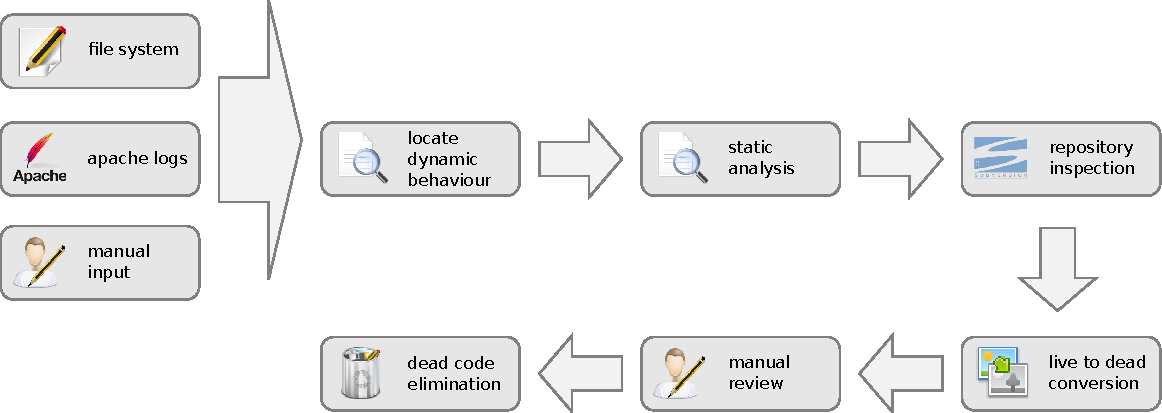
\includegraphics[scale=.8]{images/toolchain/toolchain.pdf}
\caption{The proposed tool chain}
\end{figure*}


The method will be tested on the Aurora at Hostnet. The findings will be written down in the final report.
This report will also incorporate the background from the literature used for the implemented techniques and
an log of the problems faced and their solutions.

\section{Global Planning}

The global planning in time can be read at the milestones. I have no courses left to complete. My literature assignment will be completed
before the kick off of my graduation project. 

During the project I have to make sure that the focus does not diverge to other day to day tasks or goes to side paths, but stays on the in this document defined goals and stick to the project milestones below. 

\subsection{Meetings}

At Hostnet a weekly meeting with my supervisor Stefan Lenselink will be scheduled. At the TU Delft I would like to have a two weekly
appointment with mr Gerd Gross to discuss the progress. See project organization for the contact data.

\subsection{Milestones}
\begin{itemize}
 \item 1 November Start at Hostnet
 \item 15 November Thesis proposal draft ready

 \item 21 November Detailed project planning ready
 \item 1 December Thesis proposal approved
 \item 15 December Dead File Removal implemented

 \item 1 January specification dynamic method
 \item 7 January Dynamic root set analysis implemented
  
 \item 1 February specification static method 
  \item 1 March Static Solution implemented
 
 \item 15 March Solution measured and written conclusion
 \item 2 April Presentation
\end{itemize}

\section{Project Organization}
\begin{description}
 \item [Responsible professor]  \hfill \\
  prof. dr. Arie van Deursen,\\ Mekelweg 4, 2628 CD Delft\\ Arie.vanDeursen@tudelft.nl\\+31 15 2782486              
 \item [University supervisor]  \hfill \\
 dr. Hans-Gerhard Gross\\ Mekelweg 4, 2628 CD Delft\\ h.g.gross@tudelft.nl\\+31 15 2787750              
 \item [Daily supervisor]   \hfill \\
  ir. Stefan Lenselink\\Ruyterkade 6, 1013 AA Amsterdam\\stefan@hostnet.nl\\+31 20 7500800
 \item [Student]   \hfill \\
  Hidde Boomsma, BSc\\Coenderstraat 1, 2613 SM Delft\\h.b.boomsma@student.tudelft.nl\\+31 6 48729172
\end{description}

\raggedright
\bibliographystyle{plain}
\bibliography{literature}

\end{document}
